% Auto-generated by tools/paper_race_tikz.py -- lift the tikzpicture into your IEEE paper,
% or compile this file directly (pdflatex/lualatex). Needs pgfplots >= 1.16.
\documentclass[tikz,border=2pt]{standalone}
\usepackage{pgfplots}
\pgfplotsset{compat=1.18}
\usepgfplotslibrary{groupplots,colormaps}
\definecolor{cstatic}{RGB}{153,153,153}
\definecolor{cslower}{RGB}{0,114,178}
\definecolor{cequal}{RGB}{0,158,115}
\definecolor{cfaster}{RGB}{213,94,0}
\begin{document}
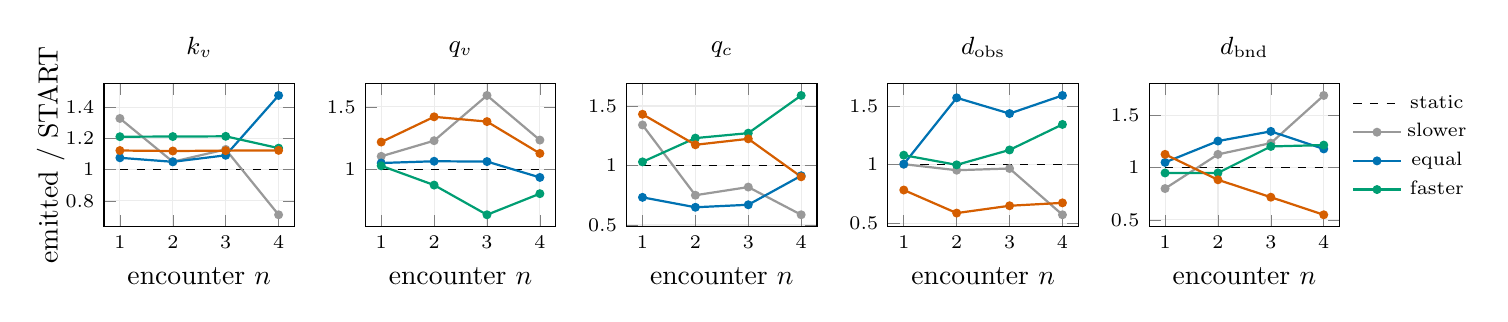
\begin{tikzpicture}
\begin{groupplot}[
  group style={group size=5 by 1, horizontal sep=0.9cm},
  width=4.0cm, height=3.4cm, xlabel={encounter $n$},
  ylabel style={font=\footnotesize}, title style={font=\small},
  tick label style={font=\scriptsize}, grid=both, grid style={gray!15},
  legend style={font=\scriptsize, draw=none, at={(1.02,1)}, anchor=north west},
  every axis y label/.style={at={(-0.28,0.5)}, rotate=90},
]
\nextgroupplot[ylabel={emitted / START}, title={$k_v$}, xtick={1,2,3,4}]
\addplot[black, dashed, line width=0.4pt, domain=1:4] {1};
\addplot[color=cstatic, mark=*, mark size=1.2pt, line width=0.8pt] coordinates {(1,1.3295) (2,1.0515) (3,1.1305) (4,0.7106)};
\addplot[color=cslower, mark=*, mark size=1.2pt, line width=0.8pt] coordinates {(1,1.0767) (2,1.0509) (3,1.0927) (4,1.4772)};
\addplot[color=cequal, mark=*, mark size=1.2pt, line width=0.8pt] coordinates {(1,1.2122) (2,1.2132) (3,1.2147) (4,1.1388)};
\addplot[color=cfaster, mark=*, mark size=1.2pt, line width=0.8pt] coordinates {(1,1.1234) (2,1.1203) (3,1.1226) (4,1.1244)};

\nextgroupplot[title={$q_v$}, xtick={1,2,3,4}]
\addplot[black, dashed, line width=0.4pt, domain=1:4] {1};
\addplot[color=cstatic, mark=*, mark size=1.2pt, line width=0.8pt] coordinates {(1,1.1033) (2,1.2285) (3,1.5911) (4,1.2334)};
\addplot[color=cslower, mark=*, mark size=1.2pt, line width=0.8pt] coordinates {(1,1.0497) (2,1.0637) (3,1.0613) (4,0.9342)};
\addplot[color=cequal, mark=*, mark size=1.2pt, line width=0.8pt] coordinates {(1,1.0275) (2,0.8728) (3,0.6348) (4,0.8040)};
\addplot[color=cfaster, mark=*, mark size=1.2pt, line width=0.8pt] coordinates {(1,1.2176) (2,1.4199) (3,1.3817) (4,1.1264)};

\nextgroupplot[title={$q_c$}, xtick={1,2,3,4}]
\addplot[black, dashed, line width=0.4pt, domain=1:4] {1};
\addplot[color=cstatic, mark=*, mark size=1.2pt, line width=0.8pt] coordinates {(1,1.3410) (2,0.7501) (3,0.8187) (4,0.5857)};
\addplot[color=cslower, mark=*, mark size=1.2pt, line width=0.8pt] coordinates {(1,0.7323) (2,0.6488) (3,0.6699) (4,0.9141)};
\addplot[color=cequal, mark=*, mark size=1.2pt, line width=0.8pt] coordinates {(1,1.0305) (2,1.2305) (3,1.2722) (4,1.5890)};
\addplot[color=cfaster, mark=*, mark size=1.2pt, line width=0.8pt] coordinates {(1,1.4309) (2,1.1742) (3,1.2243) (4,0.9051)};

\nextgroupplot[title={$d_\mathrm{obs}$}, xtick={1,2,3,4}]
\addplot[black, dashed, line width=0.4pt, domain=1:4] {1};
\addplot[color=cstatic, mark=*, mark size=1.2pt, line width=0.8pt] coordinates {(1,1.0044) (2,0.9527) (3,0.9674) (4,0.5712)};
\addplot[color=cslower, mark=*, mark size=1.2pt, line width=0.8pt] coordinates {(1,1.0049) (2,1.5728) (3,1.4379) (4,1.5930)};
\addplot[color=cequal, mark=*, mark size=1.2pt, line width=0.8pt] coordinates {(1,1.0816) (2,0.9987) (3,1.1264) (4,1.3449)};
\addplot[color=cfaster, mark=*, mark size=1.2pt, line width=0.8pt] coordinates {(1,0.7832) (2,0.5857) (3,0.6484) (4,0.6732)};

\nextgroupplot[title={$d_\mathrm{bnd}$}, xtick={1,2,3,4}]
\addplot[black, dashed, line width=0.4pt, domain=1:4] {1};
\addplot[color=cstatic, mark=*, mark size=1.2pt, line width=0.8pt] coordinates {(1,0.8001) (2,1.1278) (3,1.2355) (4,1.6920)};
\addplot[color=cslower, mark=*, mark size=1.2pt, line width=0.8pt] coordinates {(1,1.0508) (2,1.2552) (3,1.3479) (4,1.1799)};
\addplot[color=cequal, mark=*, mark size=1.2pt, line width=0.8pt] coordinates {(1,0.9495) (2,0.9501) (3,1.2036) (4,1.2166)};
\addplot[color=cfaster, mark=*, mark size=1.2pt, line width=0.8pt] coordinates {(1,1.1280) (2,0.8842) (3,0.7173) (4,0.5490)};
\legend{static,slower,equal,faster}
\end{groupplot}
\end{tikzpicture}
\end{document}
